% tables/literature_review/interest_indicators.tex
\begin{table}[H]
    \centering
    \scriptsize % Make the text smaller
    \begin{tabular}{|M{2cm}|M{2cm}|M{8cm}|}
        \hline
        \textbf{Example function}   & \textbf{Interest indicator}     & \textbf{DQ control operator pattern}                                              \\ \hline
        \textbf{$current\_value()$} & Extraordinary value ranges      & 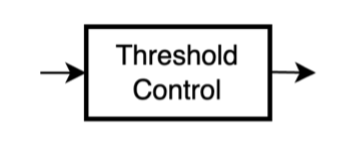
\includegraphics[scale=0.75]{figures/literature_review/interest_indicators_1.png} \\ \hline
        \textbf{$sliding\_slope()$} & Extraordinary value alterations & 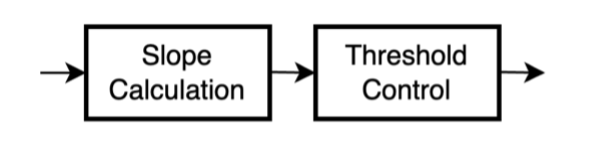
\includegraphics[scale=0.75]{figures/literature_review/interest_indicators_2.png} \\ \hline
        \textbf{$fft\_slope()$}     & Changing periodicity            & 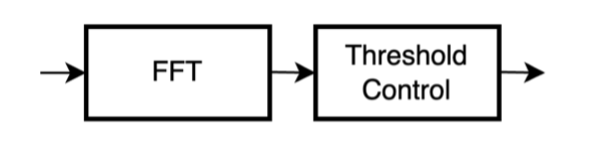
\includegraphics[scale=0.75]{figures/literature_review/interest_indicators_3.png} \\ \hline
        \textbf{$fft()$}            & Unsteadiness                    & 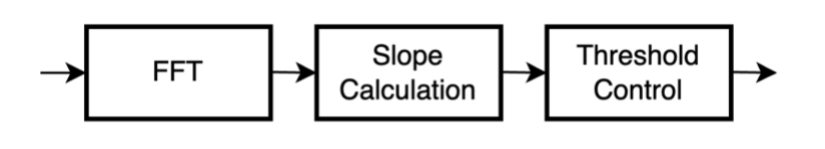
\includegraphics[scale=0.75]{figures/literature_review/interest_indicators_4.png} \\ \hline
    \end{tabular}
    \caption{Interest indicators and operators (Klein and Lehner 2009)}
    \label{table:interest_indicators}
\end{table}